% Beamer template
% Author: Ozgur Taylan TURAN
% Delft University of Technology

\documentclass[aspectratio=169]{beamer}

% PACKAGES
\usepackage[english]{babel}
\usepackage{graphicx}
\usepackage{animate}
%\usepackage{calc}
\usepackage{calligra}
\usepackage[absolute,overlay]{textpos}
\usepackage[T1]{fontenc}
%\usefonttheme{serif}
\usefonttheme{professionalfonts}
\usepackage{amsmath}
\usepackage{palatino}
\usepackage{mathpazo}
\usepackage{graphicx}
%\usepackage{subfig}
\usepackage{tikz}
\usetikzlibrary{shapes,arrows}
\usepackage{xcolor}
\usepackage[T1]{fontenc}
%\usefonttheme{serif}
%\usepackage{titling}
\usepackage{graphicx}
%\usepackage{subfig}
%\usepackage{tikz}
%\usetikzlibrary{shapes,arrows}
\usepackage{mathtools}
% TIKZ STYLES
\tikzstyle{decision} = [diamond, draw, 
    text width=4.5em, text badly centered, node distance=3cm, inner sep=0pt]
\tikzstyle{block} = [rectangle, draw, 
    text width=4em, text centered, rounded corners, minimum height=4em, node distance=3cm]
\tikzstyle{line} = [draw, -latex']
\tikzstyle{cloud} = [draw, ellipse, node distance=3cm,
    minimum height=2em]
    
% BIB SETTINGS
\usepackage[backend=bibtex,firstinits=true,maxnames=30,maxcitenames=20,url=false,style=authoryear]{biblatex}
%\bibliography{../../../Mendeley/bibtex/Intro}
\bibliography{bibli.bib}
%\bibliography{../../Dropbox/Mendeley/bibtex/FEM-Intro}

\setlength\bibitemsep{0.3cm} % space between entries in the reference list
\renewcommand{\bibfont}{\normalfont\scriptsize}
\setbeamerfont{footnote}{size=\tiny}
\renewcommand{\cite}[1]{\footnote<.->[frame]{\fullcite{#1}}}
\setbeamertemplate{bibliography item}{}

% NAVIGATION
\setbeamertemplate{navigation symbols}{} % remove navigation symbols


\mode<presentation>{\usetheme{tot}}

 % COVER PAGE INFO   
\newcommand{\mytitle}{\color{White}\huge{\textbf{PR Lab Discussion}}}
\newcommand{\myauthor}{\color{White}\textcalligra{\LARGE Ozgur Taylan Turan}}
\newcommand{\authorlabel}{\small O.T. Turan}
\author{\authorlabel}


\begin{document}
% COVER PAGE
{
{
\def\beamer@entrycode{\vspace*{-\headheight}}
\setbeamertemplate{frametitle}[default][center]
\setbeamertemplate{navigation symbols}{}
\usebackgroundtemplate{
\includegraphics[width=\paperwidth,height=\paperheight]{cover/coverart.pdf}}

\begin{frame}[plain] 

\begin{minipage}{\textwidth}
	\centering{\mytitle} \\
	%\vspace{1cm}
	%\centering{\mysubtitle} \\
	\vspace{1cm}
	\centering{\color{White}November 15, 2021} \\
	\vspace{1cm}
	\centering{\myauthor}\\
\end{minipage}
\end{frame}
}

\setbeamercovered{transparent}
\setbeamertemplate{footline}{\usebeamertemplate*{minimal footline}}
\setbeamertemplate{headline}{\usebeamertemplate*{minimal headline}}
\def\beamer@entrycode{\vspace*{-\headheight}}
}
% MAIN
{\setbeamertemplate{footline}{\usebeamertemplate*{minimal footline}}

}
\setbeamercovered{transparent}


\begin{frame}
	\centering
	\color{Pink}{Proprietary Software Usage in Research}	
\end{frame}

\begin{frame}{What led me to this topic?}
	\centering
	\begin{minipage}{0.6\textwidth}
		\begin{itemize}
			\item Industry \& science $\to$ Industrialized Science?
		\end{itemize}
	\end{minipage}%
	\begin{minipage}{0.4\textwidth}
		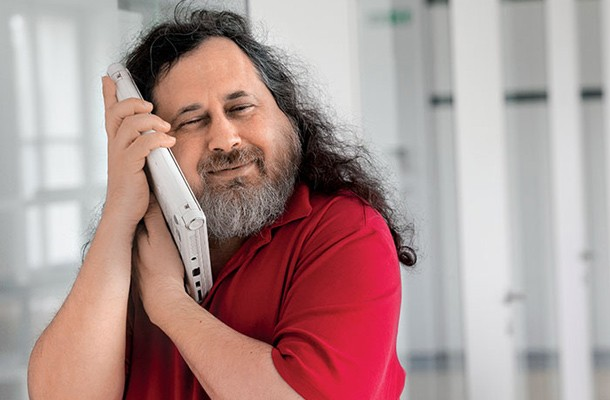
\includegraphics[width=\textwidth]{Figures/Richard-Stallman}\cite{richard}	
	\end{minipage}
\end{frame}


\begin{frame}{Open-science\cite{UNESCO} $\to$ Open-source vs Free Software}
	\begin{minipage}{0.6\textwidth}
	\begin{itemize}
		\item Hype train? 
	\end{itemize}
	\end{minipage}%
	\begin{minipage}{0.4\textwidth}
		\centering
		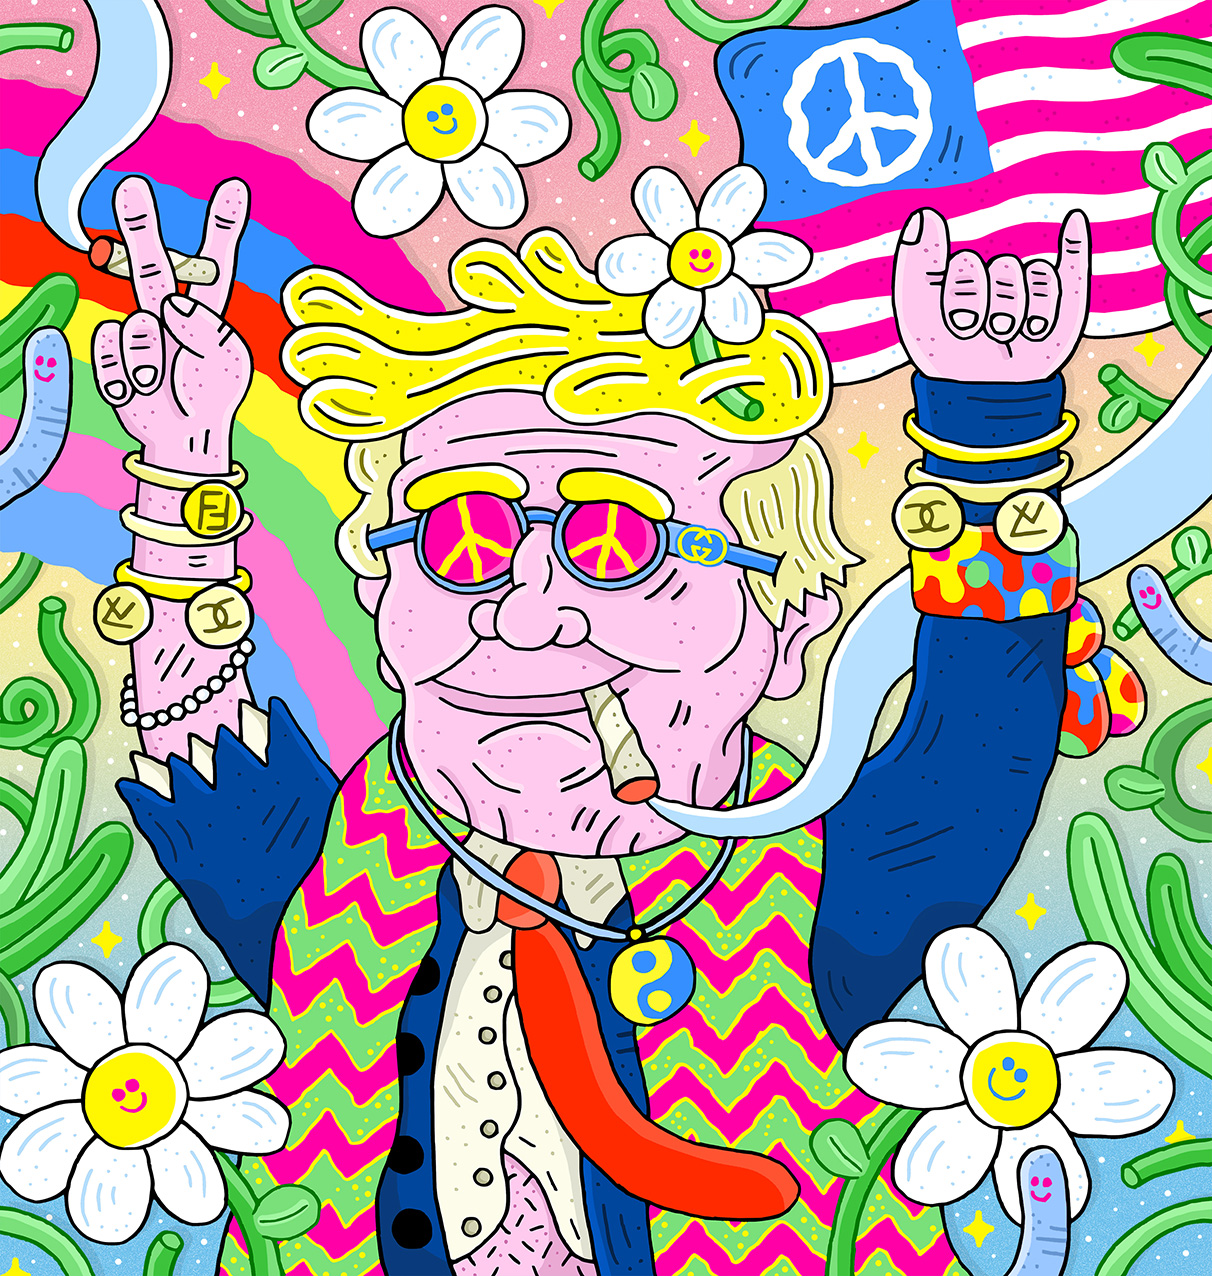
\includegraphics[width=0.9\textwidth]{Figures/hippy}\cite{Sam}
	\end{minipage}
\end{frame}

\begin{frame}{Proprietary Software}
	
	\begin{minipage}{0.5\textwidth}
		\begin{itemize}
			\item Scientific value
			\item Reproducibility
			\item Pressure on researchers
		\end{itemize}
	\end{minipage}%
	\begin{minipage}{0.5\textwidth}
		\centering
		\color{Pink}Your thoughts?
	\end{minipage}
\end{frame}




\end{document}